\documentclass[a4paper]{article}

\usepackage[utf8]{inputenc}
\usepackage[portuges]{babel}
\usepackage{graphicx}
\usepackage{fancyvrb}

\title{Projeto de Laboratórios de Informática 1\\Grupo li1g030}
\author{Miguel Quaresma A77049}

\begin{document}

\maketitle

\begin{abstract}

Este relatório tem o objetivo de retratar e refletir sobre o processo de desenvolvimento do jogo Sokoban recorrendo à linguagem de programação \textit{Haskell}, no âmbito da UC de Laboratórios de Informática I. Este projeto, de média dimensão, compreendeu duas fases de avaliação, sendo que cada uma se encontrava dividida em três tarefas distintas que iriam facilitar a concepção do jogo, divindo a mesma nas suas partes mais elementares. 
Para analisar o processo de desenvolvimento do jogo, o relatório que se segue irá focar-se nos aspetos fulcrais do jogo, nomeadamente as estratégias utilizadas na sua programação, os problemas encontrados e a forma de resolução dos mesmos bem como o produto final, ou seja, o jogo acabado. 

\end{abstract}

\tableofcontents

\section{Introdução}
\label{sec:intro}

O objetivo inicial deste projeto é o desenvolvimento de um jogo que se assemelhe ao presente em \textit{Sokoban.info}, recorrendo para isso à linguagem Haskell. A realização deste projeto possiblitou aos seus intervenientes um aprofundar do seu conhecimento relativo à linguagem de programação (funcional) Haskell, ao estimular a consulta da documentação e a implementação de soluções face a problemas que surgiram durante o processo de desenvolvimento. Para tal, foi proposto aos alunos que realizassem 6 tarefas computacionais distintas, cada uma com foco em diferentes aspetos de programação, nomeadamente a validação de um mapa ou o design de uma interface gráfica. Esta característica facilitou a concepção do jogo, visto que permitiu a divisão da mesma em partes mais pequenas e mais simples de resolver, algo fundamental em programação. Sendo assim, quando se tratou da "realização" do jogo em si, a maior parte do trabalho encontrava-se feito, sendo apenas necessário implementar todas as tarefas realizadas em conjunto, adicionando alguns extras.

Por forma a facilitar a compreenssão do processo de desenvolvimento, este relatório encontra-se repartido da seguinte forma:
\begin{description}
	\item [Secção ~\ref{sec:problema} ] : onde se procede à descrição do problema em mãos
	\item [Secção ~\ref{sec:solucao} ] : na qual se relata a forma encontrada para a realização do projeto
	\item [Secção ~\ref{sec:conclusao} ] : onde se apresentam algumas reflexões referentes ao projeto
\end{description}


\section{Descrição do Problema}
\label{sec:problema}

O projeto em questão teve como intuito principal o desenvolvimento de um jogo semelhante ao presente em \textit{Sokoban.info}. Para tal o mesmo foi dividido em duas fases, cada uma compreendendo três tarefas (para um total de 6) enumeradas a seguir:	 
	\begin{enumerate}
		\item Validação de um Mapa (recebido na forma de ficheiro de texto)
		\item Simplificação do mapa e colocação do boneco e das caixas 
		\item Validação de um movimento por parte de um boneco e \textit{output} do resultado
		\item Execução de uma sequência de movimentos
		\item Cálculo da área (envolvente) de uma \textbf{Picture}
		\item Desenvolvimento da \textit{interface} gráfica e compilação de todas as tarefas anteriores 
	\end{enumerate}

\subsection{Fase 1}
A primeira tarefa consistia em receber, como \textit{input}, um mapa sob a forma de um ficheiro de texto e validar o mesmo, verificando os caracteres e as coordenadas fornecidas.

\begin{figure}[ht]
	\centering
	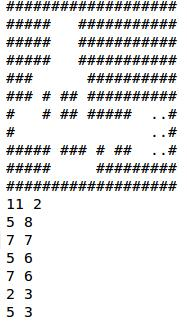
\includegraphics[width=0.2\textwidth]{assets/mapaExemplo.jpg}  
	\caption{Ficheiro de Input da tarefa 1}
\end{figure}


A tarefa seguinte consistia em remover as paredes (cardinais) redudantes e colocar as caixas e o boneco recorrendo às coordenadas dadas, fazendo output do resultado.

O objetivo da terceira tarefa era receber o mesmo ficheiro de mapa mas com um caracter no fim, que indicava a direção em que se pretendia que o boneco se movimentasse, sendo depois necessário validar esse mesmo movimento e fazer output das novas coordenadas do boneco.

\begin{figure}[ht]
	\centering
	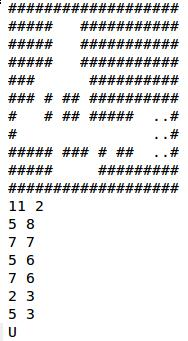
\includegraphics[width=0.2\textwidth]{assets/mapaMovimento.jpg}
	\caption{Ficheiro de Input da tarefa 2}
\end{figure}

\subsection{Fase 2}
A primeira tarefa desta fase era um prolongamento da última tarefa da fase anterior, que consistia em receber não um, mas uma série de movimentos, validando-os todos, sendo que o output correspondia ao número de movimentos válidos realizados pelo boneco, bem como o estado do mapa após os mesmos, ou seja, se este se encontrava completo ou não.

A penúltima tarefa do projeto representou uma introdução ao uso do \emph{Gloss}, a biblioteca gráfica do Haskell. Nesta tarefa o objetivo era calcular a menor área envolvente de uma \textbf{Picture}. 

Por fim, a última tarefa consistia em implementar uma \textit{interface} gráfica bem como as mecânicas fundamentais do jogo, sendo que esta tarefa tinha uma componente mais criativa, em que os alunos podiam implementar diferentes aspetos do jogo, como a escolha de bonecos ou de mapas, entre outros.


\section{Concepção da Solução}
\label{sec:solucao}

\subsection{Estruturas de Dados}

As estruturas de dados, como o próprio nome indica, são a forma principal de armazenar e manipular dados, tendo por isso um papel fulcral no trabalho. De todos os tipos existentes na linguagem Haskell destacam-se, de seguida, aquelas que mais relevo tiveram na realização do trabalho:
\begin{description}
		\item [\textbf 	{Strings}] : sendo exemplo destas o conteúdo dos ficheiro de texto contendo os mapas, também designadas de listas de caracteres
		\item [\textbf 	{[(Float, Float)]} / \textbf {[(Int, Int)]}] : usados no armazenamento de coordenadas ou no controlo dos movimentos do boneco
		\item [\textbf 	{Pictures}] : responsáveis pela composição da \textit{interface} gráfica
		\item [\textbf {Events}] : possíves \textit{inputs} através do teclado, rato, etc
\end{description}

	
\subsection{Implementação}


\subsubsection{Fase 1}
Inicialmente focámo-nos na realização das diversas tarefas propostas, já que isto iria facilitar a conclusão do projeto final. Com isso em mente, a primeira tarefa consistia em receber um ficheiro de texto contendo o mapa e as coordenadas das caixas e validá-lo, verificando se todos os caracteres nele incluídos eram válidos e se as coordenadas eram também elas válidas.

O objetivo seguinte era receber o mesmo ficheiro de texto, mas desta vez com o intuito de simplificar o mapa, retirando os cardinais que se revelassem redundantes e colocando o boneco e as caixas nos locais indicados pelas coordenadas, fazendo o \textit{output} do resultado correspondente. Nesta tarefa, a maior dificuldade encontrada foi a de identificar os cardinais redundantes, que acabou por ser ultrapassada ao analisarmos todos os cardinais do mapa e os caracteres envolventes, por forma a decidir se o cardinal em questão era necessário no contexto em que se encontrava.

Por fim, era necessário receber um ficheiro idêntico ao anterior mas com um caracter depois das coordenadas, caracter este que indicava a direção do movimento do boneco ('U'-cima, 'D'-baixo, 'L'-esquerda, 'R'-direita), que tinha que ser avaliado quanto à sua validade no contexto e fazer output das coordenadas do boneco consoante a validade e, em caso positivo, a direção do movimento.

\subsubsection{Fase 2}
Nesta fase inicou-se então o desenvolvimento das mecânicas que permitem ao utilizador interagir com o jogo desenvolvido.
Para tal, e como continuação da última tarefa realizada, tinha-se como objetivo receber um ficheiro de texto com um mapa e, desta vez, com um conjunto de caracteres indicando a direção em que se pretendia que o boneco se movesse, sendo que o resultado desta vez seria o número de movimentos válidos realizados e o estado do mapa após estes movimentos, ou seja, se este se encontrava incompleto ou completo. Um dos obstáculos encontrado foi a verificação do estado do mapa. A solução encontrada para este problema foi verificar se, após cada movimento, ainda havia H's no mapa, visto que estes simbolizam caixas que ainda não se encontram na posição final. Isto foi conseguido através da seguinte função:
\begin{verbatim}
caixasF :: [String] -> Bool
caixasF [] = True
caixasF (h:t) = if(aux h) then caixasF t else False
	where
		aux :: String -> Bool
		aux [] = True
		aux (h:t) = if(h == 'H') then False else aux t
\end{verbatim}

Na tarefa seguinte tivemos o primeiro contacto com o \emph{Gloss}, a biblioteca gráfica do \textit{Haskell}. O que nos era requerido era implementar um programa que, ao receber uma \textbf{Picture} como \textit{input}, calculasse as medidas do retângulo envolvente da mesma. A principal dificuldade foi o cáculo destas medidas quando o \emph{Circle} (círculo) era a figura em questão. Por forma a ultrapassar esta mesma dificuldade, decidimos obter as coordenadas de vários pontos do círculo, visto que isto tornaria mais preciso o resultado que obtíamos. Para tal, usamos a função \emph{map} sobre uma lista de compreensão, da seguinte forma:
\begin{verbatim}
pontosCirculo :: Float -> Path
pontosCirculo r = map (\x -> (sin(x) * r, cos(x) * r)) l
		where
			l = [5,10..360]
\end{verbatim}

Na útlima tarefa iniciámos então o desenvolvimento do jogo em si, recorrendo para isso ao trabalho anteriormente realizado, bem como à implementação de uma \textit{interface} gráfica e de um sistema que permitisse ao utilizador controlar o boneco. Para isso recorremos à função \emph{reageManager} que consoante o comportamento do utilizador, reagia em conformidade. Isto era conseguido através de \textbf{Events}, para os quais definimos uma reação por parte do jogo. Exemplo disto era o caso em que o utilizador premia a tecla 'r', altura em que o mapa em que o utilizador se encontrava voltava ao estado inicial. Para conseguir esta funcionalidade, recorremos à função anteriormente referida, que "guardava uma cópia" do estado inicial do mapa, e que, aquando da ocorrência do evento referido, passava este estado como parâmetro à função \emph{desenhaMapa}. Para testar os movimentos, ou melhor, a sua validade, recorremos a uma função semelhante à implementado na tarefa 3, modificando-a de maneira a que esta se enquadrasse no contexto em que era utilizada. 
Para tornar o jogo um pouco diferente, e tendo em conta que este era um dos aspetos avaliados, escolhemos os \emph{Simpsons} como tema do jogo e demos a opção ao utilizador de escolher entre quatro escolhas de bonecos diferentes, bem como diferentes mapas. A escolha dos bonecos alterava não só o boneco em si, mas também aquilo que este tem que empurrar/arrumar. 

\begin{figure}[ht]
	\centering
	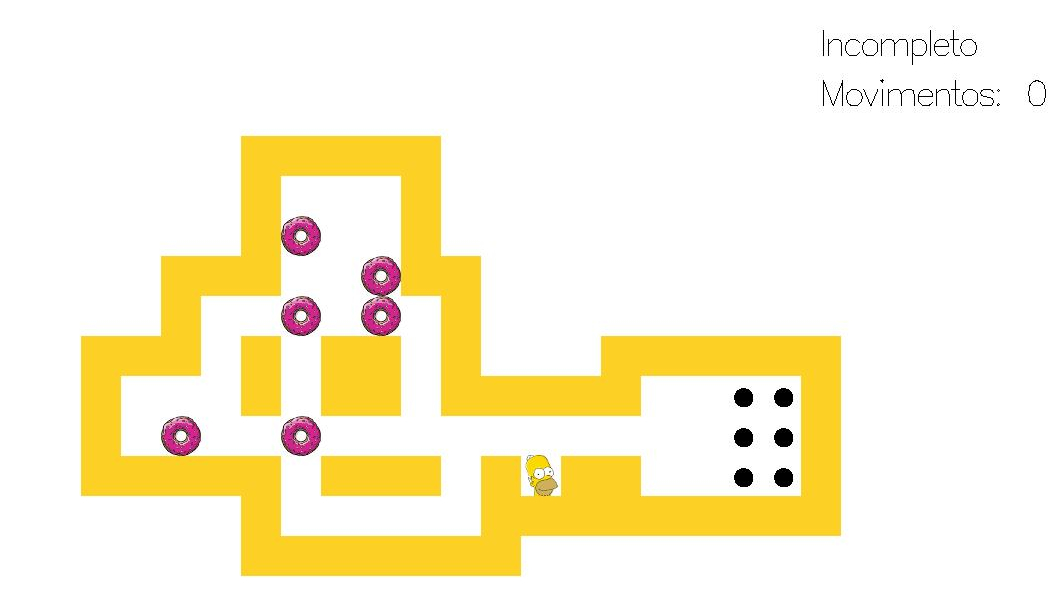
\includegraphics[width=0.45\textwidth]{assets/escolha1.jpg}
	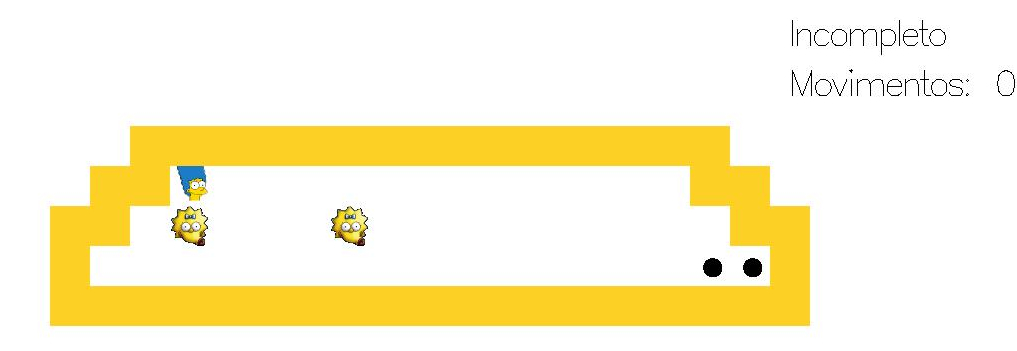
\includegraphics[width=0.45\textwidth]{assets/escolha2.jpg}  
	\caption{Resultado de escolher os bonecos}
\end{figure}

Por fim adicionamos um contador de movimentos, que controla o número de movimentos válidos realizados pelo utilizador, e um ecrã de congratulação ao utilizador após o término do jogo.

\begin{figure}[ht]
	\centering
	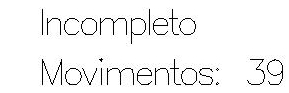
\includegraphics[width=0.45\textwidth]{assets/contadorMovimentos.jpg} 
	\caption{Registo de movimentos}
	 
\includegraphics[width=0.45\textwidth]{assets/final.jpg} 
	 \caption{Fim do jogo}
\end{figure}

\subsection{Testes}

Após e durante a realização de cada uma das tarefas propostas, o teste do trabalho desenvolvido revelou ser um dos aspetos mais importantes a ter em conta, visto que este permitia avaliar o código e encontrar possíveis erros na forma como corria. Esta avaliação podia ser realizada com conhecimento do código em questão (\textit{White-Box testing}), possiblitando assim a identificação de eventuais redundâncias no mesmo ou, se fosse realizado sem o conhecimento do código (\textit{Black-box testing}), permitia realizar uma avaliação de desempenho face a diversos testes definidos pelos alunos. Por forma a facilitar a avaliação do código com o uso de testes, recorreu-se à implementação de uma função que corresse estes testes automaticamente, e que apresentasse o resultado dos mesmos:

\begin{figure}[ht]
	\centering
	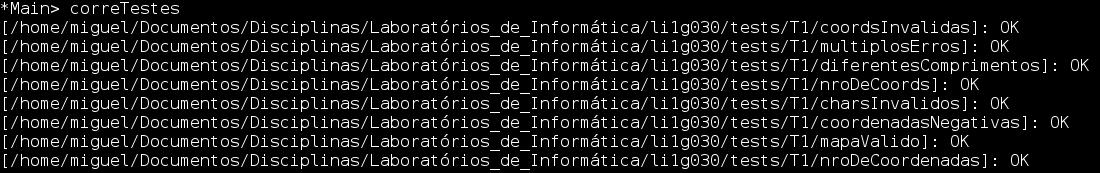
\includegraphics[width=0.75\textwidth]{assets/testeExemplo.jpg}
	\caption{Output da função \emph{correTestes}}
\end{figure}

Para avaliar o jogo desenvolvido, e visto que os testes anteriormente referidos não se aplicavam neste contexto, optámos por ir testando o trabalho à medida que este era desenvolvido, visto que isto nos permitia focarmo-nos apenas nos aspetos novos e identificar possíveis falhas nessas partes. 

\section{Conclusões}
\label{sec:conclusao}

Em resumo, consideramos que os objetivos principais foram atingidos, apesar de alguns aspetos não terem sido implementados da forma incialmente pretendida e de outros se terem revelado mais difíceis de realizar do que o inicialmente calculado. Por outro lado, houve certas características do projeto que gostariamos de ter conseguido implementar, mas que, dada a sua complexidade, não foi possível. Sendo exemplo disto o uso de um registo dos "\textit{scores}" obtidos e, caso o utilizador alcançasse um número de movimentos record, a congratulação pelo feito. 

\end{document}
